\documentclass[output=paper]{langscibook}

\author{Dorota Klimek-Jankowska\affiliation{University of Wrocław} and Joanna Błaszczak\affiliation{University of Wrocław}}
\title[Number semantics and the interpretation of imperfective verbs in Polish]{Implications of the number semantics of NP objects for the interpretation of imperfective verbs in Polish}  
\abstract{Languages differ in the range of readings of imperfective aspect but its single ongoing and plural event readings are cross-linguistically licensed. In this study we focus on the role of the number of NP objects on the disambiguation of Polish imperfective verbs. The crucial observation is that a singular object may block whereas a plural NP object creates a strong preference for the plural event reading of imperfective verbs. However, in the right context, the plural event reading of imperfective verbs is also available with singular NP objects. In order to account for these observations, we combine underspecification and number approaches to imperfective aspect and we propose that imperfective is underspecified for number and this information is specified via a coercion template mainly on the basis of the number semantics of nominal objects of imperfective verbs.

\keywords{imperfective aspect, semantic underspecification, number, contextual cues, gradual specification process}}

\begin{document}
\SetupAffiliations{mark style=none}
\maketitle

\section{Introduction}\label{jan-bla:fansb:kb:sec1}

It is known from the literature on English that the number of an (indefinite) NP object has an impact on the VP interpretation. For example, while in a sentence with a singular indefinite object a predicate like \textit{eat} receives a telic interpretation (cf. \textit{John ate an apple}), the use of a plural indefinite object results in an atelic interpretation (cf. \textit{John ate apples}). The readings in question are associated with lexical aspect (ibidem).\footnote{For space reasons, we will not go into the discussion of the composition of semantic aspect in English. The reader is referred to \citet{Filip1994}; \citet{Krifka1989,Krifka1992,Krifka1998}; \citet{Rothstein2004}; \citet{Verkuyl1972,Verkuyl1993,Verkuyl1999}. For further discussion, see \citet{Dowty1979,MacDonald2008,Tenny1994,Willim2006}; and the references cited there.} What is less known is the role of the number of an NP object on the interpretation of the verbal predicate in languages with grammatical aspect such as Polish (or other Slavic languages).\footnote{Semantic/lexical aspect (also referred to as “situational aspect” or “situation type,” “eventuality type,” “Vendlerian aspect,” “inner aspect,” or “Aktionsart”) is lexically encoded in a verbal predicate. Grammatical/morphological aspect (also referred to as “viewpoint aspect” or “outer aspect”), on the other, is conveyed by “a grammatical morpheme, usually verbal” \citep[2]{Smith1997}.} In the present paper we will focus on the role of the number of an NP object on the interpretation of an imperfective verb in Polish. The usual assumption is that imperfective predicates reflect the perspective of an ``insider'', who sees a portion of an event from the inside and is oblivious to its endpoints (\citealt{KazaninaandPhillips2003}). In more formal terms, the imperfective introduces the inclusion relation between the event time interval and reference time interval, where the former includes the latter, leaving the potential endpoints of an event from view; cf. \REF{jan-bla:fansb:kb:ex1} (for more discussion see, among others, \citealt{Borik20022006}; \citealt{Comrie1976}; \citealt{KampandReyle1993}; \citealt{Klein1994}; \citealt{Reichenbach1947}; \citealt{Smith1997}).

\ea \sib{\textsc{ipfv}} $= \lambda P. \lambda t. \exists e : \tau(e) \supseteq t \wedge P(e)$\label{jan-bla:fansb:kb:ex1}
\z

\noindent It has been noticed in the literature that in those languages which distinguish between perfective and imperfective aspect, imperfective is multiply ambiguous (see \citealt {ArreguiRiveroandSalanova2014}; \citealt{CipriaandRoberts2000}; \citealt{Deo2009,Deo2015}; \citealt{Hacquard2006}; \citealt{deSwart1998}). However, what seems to be the case is that even if languages differ in the range of possible readings of imperfective, two meanings of imperfective aspect can be identified as standard cross-linguistically. The readings in question are single ongoing and plural event readings, illustrated by the Polish examples in \REF{jan-bla:fansb:kb:ex2} and \REF{jan-bla:fansb:kb:ex3}, respectively.

\ea Single ongoing\label{jan-bla:fansb:kb:ex2}\\
\gll Anna czytała gazetę, kiedy ktoś wszedł do domu.\\  
     Anna read.\textsc{ipfv}.\textsc{pst}.\textsc{3sg}.\textsc{f} newspaper.\textsc{acc} when someone enter.\textsc{pfv}.\textsc{pst}.\textsc{3sg}.\textsc{m} into house\\
\glt ‘Anna was reading a newspaper when someone entered the house.’
\z

\ea Plural event reading\label{jan-bla:fansb:kb:ex3}\\
Maria prasowała ubrania córki wieczorami.\\  
Mary iron.\textsc{ipfv}.\textsc{pst}\textsc{3sg}.\textsc{f} clothes.\textsc{acc} daughter.\textsc{gen} evenings.\textsc{ins}\\
\glt ‘Mary ironed her daughter’s clothes in the evenings.’
\z

\noindent On its single ongoing reading (ex. \REF{jan-bla:fansb:kb:ex2}), the imperfective verb refers to an event which is incomplete at the asserted interval \citet[200--201]{Willim2006}. By contrast, on the plural event reading, the imperfective verb most typically refers to a series of delimited events happening on several occasions, as in \REF{jan-bla:fansb:kb:ex3}. Interestingly, it seems to be the case that the availability of a given reading of the imperfective verb in Polish might be blocked or facilitated depending on what kind of object, singular or plural, is used. Examples in \REF{jan-bla:fansb:kb:ex4} and \REF{jan-bla:fansb:kb:ex5} illustrate this point.

\ea
\gll Rubens malował kobietę.\label{jan-bla:fansb:kb:ex4}\\  
     Rubens paint.\textsc{ipfv}.\textsc{pst}.\textsc{3sg}.\textsc{m} woman.\textsc{sg}.\textsc{acc}\\
\glt ‘Rubens was painting a woman.’
\z

\ea
\gll Rubens malował kobiety.\label{jan-bla:fansb:kb:ex5}\\  
     Rubens paint.\textsc{ipfv}.\textsc{pst}.\textsc{3sg}.\textsc{m} woman.\textsc{pl}.\textsc{acc}\\
\glt ‘Rubens painted women.’
\z

\noindent In \REF{jan-bla:fansb:kb:ex4}, in which a singular (indefinite NP object) is used, the imperfective predicate denotes a single ongoing eventuality.\footnote{In Polish, there is no indefinite marking in NPs but the indefinite/definite reading of bare singular nouns is determined by the information structure. More precisely, under normal intonation the sentence stress falls on the final element, that is, the default placement of the focus exponent in Slavic is in the right periphery of a sentence (see \citealt{Junghanns2002}).}\textsuperscript{,}\footnote{In principle it is pragmatically possible that one paints the same woman again and again but in the context with Rubens, who is well known for painting different women on different occasions, the reading that he painted the same woman on different occasions is pragmatically implausible. According to our intuitions and the intuitions of the native speakers consulted the plural event reading in this context is not available. Moreover, even if you use a different subject in \REF{jan-bla:fansb:kb:ex4}, e.g., Peter, still the plural event reading is very hard (if not impossible) to obtain.} Crucially, the plural event reading is blocked in this case. However, when we change the grammatical number of the NP object in \REF{jan-bla:fansb:kb:ex5} to plural, the plural event reading becomes available. The above examples demonstrate that the number of an NP object plays an important role for the interpretation of an imperfective verb in Polish. But this is not the end of the story yet since in the right context, the plural event reading of imperfective verbs is also available with singular NP objects. Take \REF{jan-bla:fansb:kb:ex6} as an example.

\ea
\gll Audrey Hepburn paliła fajkę.\label{jan-bla:fansb:kb:ex6}\\  
     Audrey Hepburn smoke.\textsc{ipfv}.\textsc{pst}.\textsc{3sg}.\textsc{f} pipe.\textsc{sg}.\textsc{acc}\\
\glt ‘Audrey Hepburn smoked a tobacco pipe.’
\z

\noindent In \REF{jan-bla:fansb:kb:ex6} the most natural interpretation is that she smoked a tobacco pipe (possibly the same tobacco pipe) on several occasions. In order to account for these observations, we will rely on \citeauthor{Ferreira2004}'s (\citeyear{Ferreira2004, Ferreira2005}) number approach to imperfective aspect, according to which it selects for either a singular or plural VP. \citeauthor{Kagan2008}'s (\citeyear{Kagan2008, Kagan2010}) treatment of imperfective aspect as plural on events will also be discussed in this connection. We will also adopt \citeposst{deSwart2006} notion of bijection, which allows for a dependent reading between pairs of individuals and events in plural sets. We will argue that imperfective is underspecified for number and this information is specified via \citeposst{Dolling2014} coercion template mainly on the basis of the number semantics of nominal objects of imperfective verbs.

The paper is organized in the following way. First, in \sectref{jan-bla:fansb:kb:sec2} we will present the underspecification approach to imperfective aspect. We will argue that the underspecification approach alone is not able to capture some crucial facts related to the interaction of imperfective aspect and the number of the NP objects. Next, \sectref{jan-bla:fansb:kb:sec3} presents the results of an online questionnaire testing meaning preferences for imperfective verbs in Polish. The results of the questionnaire will speak in favor of the number theory of imperfective aspect proposed by \citet{Ferreira2004, Ferreira2005} and presented in \sectref{jan-bla:fansb:kb:sec4}. However, it will be shown that this theory is too rigorous and it does not capture the fact that the interaction of the number semantics of imperfective aspect with the number of NP objects clearly relies on pragmatics. Based on the results of these studies and observations regarding the underspecified nature of imperfective aspect, we will argue that imperfective aspect is underspecified for number and we will present our account in \sectref{jan-bla:fansb:kb:sec5}. \sectref{jan-bla:fansb:kb:sec6} will conclude the paper.

\section{The underspecification approach to imperfective aspect}\label{jan-bla:fansb:kb:sec2}

In Polish and in most languages which manifest the distinction between perfective and imperfective aspect, the former is semantically more marked (it has a more specific meaning and a more constrained distribution) and the latter is semantically less marked (it has a wider, more general meaning and occurs in a wider set of contexts). Perfective aspect has a very specific meaning in that it denotes an episodic bounded event.
In contrast, imperfective aspect has a wider meaning in that it can be used to describe episodic unbounded, iterative or habitual eventualities. Consequently perfective aspect has a more restricted distribution than imperfective aspect.\footnote{Sometimes it is assumed that unmarked forms lack the specific meaning a marked form has (cf. \citealt{Borik20022006}, who assumes that the meaning of imperfective aspect is non-perfective).} Additionally, there is a gap in the distribution of perfective aspect. Perfective aspect can be used to talk about past and future events while imperfective aspectual forms can be used to talk about past, present and future events, as shown in 
\tabref{jan-bla:fansb:kb:tab1}.

\begin{table}
\caption{The distribution of perfective and imperfective aspect for past, present and future reference}
\label{jan-bla:fansb:kb:tab1}
 \begin{tabular}{lllll}
  \lsptoprule
            Past time reference & Present time reference & Future time reference\\
  \midrule
    imperfective aspect  &    imperfective aspect     & imperfective aspect\\
    perfective aspect &     & perfective aspect\\
  \lspbottomrule
 \end{tabular}
\end{table}

Importantly, imperfective verbs in Polish can describe events as completed in what are know as general factual contexts, presented in \REF{jan-bla:fansb:kb:ex7}.

\ea
\gll Podczas zwiedzania Barcelony jeden z turystów pyta przewodnika: Jaka spektakularna budowla. Kto ją budował / zbudował?\\  
     while visiting Barcelona one of tourists asks guide what spectacular building who her build.\textsc{ipfv}.\textsc{pst}.\textsc{3sg}.\textsc{m} {} build.\textsc{pfv}.\textsc{pst}.\textsc{3sg}.\textsc{m} \\
\glt ‘While visiting Barcelona, one of the tourists asks the guide: What a spectacular building. Who built it?’\label{jan-bla:fansb:kb:ex7}
\z

\noindent This fact is challenging for all the theories of imperfective aspect since it is not clear why imperfective is used to describe event completion even though this meaning could be better expressed by means of perfective aspect. This indicates that under some circumstances the meanings of perfective and imperfective aspect overlap. For this reason different linguists treat imperfective aspect as non-aspect, non-perfective, semantically underspecified, semantically unmarked or default (see \citealt{Battistella1990}; \citealt{Borik20022006}; \citealt{Comrie1976}; \citealt{Dahl1985}; \citealt{Filip19931999}; \citealt{Forsyth1970}; \citealt{Kagan2008, Kagan2010}; \citealt{Klein1995}; \citealt{PaslawskaandStechow2003}; \citealt{Willim2006}).

The semantically underspecified status of imperfective aspect in Polish, as described above, is compatible with the observation made in \citet{AikhenvaldandDixon1998} that in many languages only semantically underspecified aspect can be used in negative statements. In Polish, negation does not always force the use of the unmarked imperfective aspect but imperfective aspect is preferred in negative contexts with necessity modals (see \citealt{KlimekJankowskaCzypionkaWitkowskiandBłaszczak2018}).\footnote{See \citet{Kagan2008, Kagan2010} for discussion of the use of the imperfective aspect (in Russian) in downward entailing environments.}  More precisely, in positive contexts Polish speakers use two different forms, perfective and imperfective, to distinguish between single completed and repetitive events, as shown in \REF{jan-bla:fansb:kb:ex8a} and \REF{jan-bla:fansb:kb:ex9a}. In contrast, in negative contexts this distinction is neutralized in the sense that one and the same form, i.e., imperfective, is used to describe single completed and repetitive eventualities, as shown in \REF{jan-bla:fansb:kb:ex8b} and \REF{jan-bla:fansb:kb:ex9b}. Using perfective aspect in a negative context with a necessity modal sounds much less natural than using the imperfective form; see \REF{jan-bla:fansb:kb:ex8c}.

\ea\label{jan-bla:fansb:kb:ex8}
\ea \gll Musiałeś wstać.\\  
        must.\textsc{pst}.\textsc{2sg}.\textsc{m}  get.up.\textsc{pfv}.\textsc{inf}\\
\glt ‘You had to get up (once).’\label{jan-bla:fansb:kb:ex8a}
\ex \gll Nie musiałeś wstawać.\\  
        not must.\textsc{pst}.\textsc{2sg}.\textsc{m} get.up.\textsc{pfv}.\textsc{inf}\\
\glt ‘You did not have to get up (once).’\label{jan-bla:fansb:kb:ex8b}
\ex \gll Nie musiałeś wstać.\\  
        not must.\textsc{pst}.\textsc{2sg}.\textsc{m}  get.up.\textsc{pfv}.\textsc{inf}\\
\glt ‘You did not have to get up (once).’\label{jan-bla:fansb:kb:ex8c}
\z
\z

\ea\label{jan-bla:fansb:kb:ex9}
\ea \gll Musiałeś wstawać.\\  
        must.\textsc{pst}.\textsc{2sg}.\textsc{m}  get.up.\textsc{ipfv}.\textsc{inf}\\
\glt ‘You had to get up (repeatedly).’\label{jan-bla:fansb:kb:ex9a}
\ex \gll Nie musiałeś wstawać.\\  
        not must.\textsc{pst}.\textsc{2sg}.\textsc{m} get.up.\textsc{ipfv}.\textsc{inf}\\
\glt ‘You did not have to get up (repeatedly).’\label{jan-bla:fansb:kb:ex9b}
\z
\z

\noindent These observations suggest that perfective aspect is semantically specific in Polish and imperfective is semantically underspecified. How to account for the semantic underspecification of imperfective aspect in a more formal way? \citet{Hacquard2006} argues that imperfective aspect has no meaning at all and its single ongoing or plural readings are realized by covert operators \textsc{prog} or \textsc{hab}. Imperfective marking is then taken to be the reflex of the presence of these covert operators in the syntactic structure. A similar view is proposed by \citet{Frąckowiak2015}, who following \citet{Hacquard2006} claims that imperfective is a semantically vacuous morpheme whose distinct meanings are introduced by distinct, phonologically null operators.

One problem for the approach proposed by \citet{Hacquard2006} is that in Polish, imperfective aspect is used to express plural event readings in contexts whose meaning is not necessarily habitual, as shown in \REF{jan-bla:fansb:kb:ex10}:

\ea\label{jan-bla:fansb:kb:ex10}
\ea \gll Jan spotykał dzisiaj ludzi z wielu zakątków świata.\\  
       Jan met.\textsc{ipfv}.\textsc{pst}.\textsc{3sg}.\textsc{m} dzisiaj people.\textsc{acc} from many parts world.\textsc{gen}\\ 
\glt ‘John kept meeting people from different parts of the world today.’\label{jan-bla:fansb:kb:ex10a}
\ex \gll Jan dwa dni czytał różne książki. \\  
        Jan two days read.\textsc{ipfv}.\textsc{pst}.\textsc{3sg}.\textsc{m} different books.\textsc{acc}\\
\glt ‘John read different books for two days.’\label{jan-bla:fansb:kb:ex10b}
\ex \gll Zawsze kiedy mężczyźni wracali z łowów, cała wioska zbierała się przy ognisku.\\  
        always when men return.\textsc{pst}.\textsc{3pl}.\textsc{m} from hunts whole village gather.\textsc{ipfv.pst.3sg.f} \textsc{refl} by fire\\
\glt ‘You did not have to get up (once).’\label{jan-bla:fansb:kb:ex10c}
\z
\z

\noindent In \REF{jan-bla:fansb:kb:ex10a} there were several occasions of John’s meeting people from different parts of the world on a specific day (not habitually). In \REF{jan-bla:fansb:kb:ex10b} John read different books on several occasions for two days (not habitually). Finally, in \REF{jan-bla:fansb:kb:ex10c} on every occasion of the men returning from hunting, the whole village gathered by the fire. In \REF{jan-bla:fansb:kb:ex10a} and \REF{jan-bla:fansb:kb:ex10b}, imperfective is used to express a plurality of events but the events in the plural set are distributed over a relatively short temporal interval and they do not constitute a habit. In \REF{jan-bla:fansb:kb:ex10c}, the plural event reading results from the universal quantification over events by means of the adverbial quantifier \textit{zawsze} ‘always’ and it has been convincingly argued by \citet{Ferreira2004, Ferreira2005} that contexts with adverbs of quantification have a different semantics than bare habitual contexts. This shows that there are several plural event readings of imperfective aspect which cannot be captured by the semantics of the \textsc{hab} operator. Additionally, under this approach it is not immediately clear how to account for the observation that singular NP objects create a strong preference for the single ongoing interpretation of imperfective verbs and plural NP objects create a strong preference for the plural event reading of imperfective verbs as in \REF{jan-bla:fansb:kb:ex4} vs. \REF{jan-bla:fansb:kb:ex5} in Polish. 

In the next section, we present the results of our online questionnaire, which indicate that the number of NP objects has a significant impact on the interpretation of imperfective verbs in Polish. Next, in \sectref{jan-bla:fansb:kb:sec4} it will be shown how the observed facts can be accounted for using \citeauthor{Ferreira2004}'s (\citeyear{Ferreira2004, Ferreira2005}) number approach to imperfective aspect and \citeposst{deSwart2006} notion of bijection. However, it will be demonstrated that there is an important role of pragmatics in the interaction of the number of NP objects and the number semantics of imperfective verbs which can be better accounted for if the number approach is combined with the underspecification approach.

\section{An online questionnaire on the role of the NP object number on the interpretation of imperfective verbs}\label{jan-bla:fansb:kb:sec3}

\subsection{Description}\label{jan-bla:fansb:kb:sec3.1}

The goal of the reported online questionnaire was to establish whether the number of an NP complement of an imperfective verb has an impact on its preferred single ongoing or plural event meaning in Polish. We wanted to determine if there are significant differences between the interpretations for different verbal conditions: (i) imperfective verbs without any complements; (ii) imperfective verbs with singular complements; (iii) imperfective verbs with plural complements. The participants were asked to decide whether a given verb or a verb phrase referred to one event in the past or many events in the past. There was an additional option ‘It is hard to say as both meanings are possible’. The participants could choose only one of the following answer types: (i) \textit{jednokrotnie} ‘one time’; (ii) \textit{wielokrotnie} ‘many times’; (iii) \textit{trudno powiedzieć (obydwa znaczenia są możliwe)} ‘difficult to say (both meanings are acceptable)’. The exact instruction to the questionnaire is given below.\footnote{The task instruction translates as follows: 
``In the questionnaire you should decide whether a given verb or a verb phrase refers to one ongoing event in the past or to an event which happened many times in the past. There is also an option ‘difficult to say as both meanings are possible’. You should chose only one option at a time.''}

\begin{quote}
W kwestionariuszu należy zdecydować, czy dany czasownik lub fraza czasownikowa odnosi się do jednego wydarzenia ciągłego w przeszłości, czy wyraża zdarzenie, które wydrzyło się wiele razy w przeszłości. Jest też do wyboru opcja ``trudno powiedzieć, obydwa znaczenia są możliwe". Należy zawsze wybrać tylko jedną odpowiedź.
\end{quote}

The questionnaire was filled in by twenty two participants (native speakers of Polish, students from the University of Wrocław (non-linguists), age 19--24). Each participant saw 10 bare imperfective verbs (without a sentential context), 10 imperfective verbs followed by a plural NP object and 10 imperfective verbs followed by a singular NP object, as summarized in \tabref{jan-bla:fansb:kb:tab2}. All the verbs had a past tense third person singular masculine morphology. All the items in our questionnaire study involved imperfective verbs (belonging to a lexical aspectual class of accomplishments) but the imperfective aspect places the perspective time inside the temporal trace of an event and hence it excludes the endpoints from view. 

\begin{table}
\caption{Polish imperfective verbs and verb phrases used in our online questionnaire}
\label{jan-bla:fansb:kb:tab2}
 \begin{tabularx}{\textwidth}{lll}
  \lsptoprule
            imperfective verb  &    imperfective verb + NP$_\textsc{sg}$     & imperfective verb + /NP$_\textsc{pl}$\\
  \midrule
    ratował  &    testował maszynę  & zamiatał korytarze \\
    ‘(he) rescued' &    ‘(he) tested (a) machine'    & ‘(he) swept corridors'\\\tablevspace
     drukował  &   rysował portret  & wyceniał działki \\
    ‘(he) printed' &    ‘(he) painted (a) portrait'    & ‘(he) priced plots of land'\\\tablevspace
     nagrywał  &   wystawiał ocenę  & podlewał trawniki \\
    ‘(he) recorded' &    ‘(he) gaved (a) grade'    & ‘(he) watered lawns'\\\tablevspace
     pakował  &   podrabiał podpis  & sporządzał raporty \\
    ‘(he) packed' &    ‘(he) counterfeited signature'    & ‘(he) made reports'\\\tablevspace
     rozliczał  &   usuwał usterkę  & podrywał dziewczyny \\
    ‘(he) calculated' &  ‘(he) removed (a) failure'    & ‘(he) picked up girls'\\\tablevspace
     oceniał  &   uszczelniał okno  & wygłaszał wykłady \\
    ‘(he) evaluated' &  ‘(he) waterproofed (a) window'    & ‘(he) gave lectures'\\\tablevspace
    montował  &   wysyłał paczkę  & wypełniał formularze \\
    ‘(he) installed' &  ‘(he) shipped (a) package'    & ‘(he) filled in forms'\\\tablevspace
    wycinał  &   malował obraz  & ozdabiał wnętrza \\
    ‘(he) cut out' &  ‘(he) painted (a) painting'    & ‘(he) decorated interiors'\\\tablevspace
    omawiał  &   szkicował budynek  & szacował straty \\
    ‘(he) discussed' &  ‘(he) sketched (a) building'    & ‘(he) estimated losses'\\\tablevspace
    poprawiał  &   wyłudzał łapówkę  & naprawiał rowery \\
    ‘(he) corrected' &  ‘(he) extorted (a) bribe'    & ‘(he) repaired bikes'\\
  \lspbottomrule
 \end{tabularx}
\end{table}

\subsection{Results}\label{jan-bla:fansb:kb:sec3.2}

Statistical analysis was conducted in the R program on a Windows compatible PC (\citealt{RDevelopmentCoreTeam2019}). To determine the existence of the differences in the reading choices of imperfective verbs in three experimental conditions: (i) verb not followed by an object (\textsc{ipfv}), (ii) verb followed by an object in singular number (\textsc{ipfv}+NP$_\textsc{sg}$) and (iii) verb followed by an object in plural number (\textsc{ipfv}+NP$_\textsc{pl}$) a loglinear analysis using loglm function (MASS package; \citealt{VenablesRipley2002}) was performed. This analysis was chosen because the response variable (reading) was nominal. A two-way loglinear analysis produced the final model, which retained all the main effects (Condition and Reading) and a two-way interaction effect ($\text{Condition}\times\text{Reading}$). The likelihood for this model was $\chi^2(0) = 1, p =1$. Removing the interaction effect resulted in a significantly poorer model fit ($\chi^2(4) = 337.463, p < 0.0001$), which indicated that the two-way interaction effect was significant. To break-down the interaction effect, standardized residuals were examined; see \tabref{jan-bla:fansb:kb:tab3} (residuals which indicate significant differences, i.e. outside the $-1.98$ to $1.98$ range, are marked in bold). 

\begin{table}
\caption{Statistics for reading choice counts with respect to experimental conditions}
\label{jan-bla:fansb:kb:tab3}
 \begin{tabularx}{\textwidth}{lQrrr}
  \lsptoprule
  Condition & Reading&Response\\
  \midrule
     & & one time & hard to say & many times\\\tablevspace
    \textsc{ipfv} & count & 36 & 104 & 110\\
    & expected count &	76.667 & 63.333	& 112\\
    & standardized residuals & $-$\textbf{4.475} & \textbf{5.110} & $-0.189$\\\tablevspace
    \textsc{ipfv}+NP$_\textsc{sg}$ & count & 155	& 51 & 190\\
    & expected count &	67.2 &	57 & 100.8\\
    & standardized residuals & \textbf{10.711} & $-$\textbf{0.795} & $-$\textbf{8.148}\\\tablevspace
    \textsc{ipfv}+NP$_\textsc{pl}$ & count & 33 & 35 & 207\\
    & expected count &	82.133 & 69.667 & 123.2\\
    & standardized residuals & $-$\textbf{5.421} & $-$\textbf{4.153} & \textbf{7.550}\\
  \lspbottomrule
 \end{tabularx}
\end{table}

Examination of standardized residuals have shown the following differences:

\begin{enumerate}
\item If the verb is not followed by any object NP (\textsc{ipfv}), respondents preferred to choose the meaning when both ‘one time’ and ‘many times’ interpretations were possible. They also avoided selecting the ‘one time’ interpretation.
\item If the verb is followed by an object in singular number, the preferred reading is the one in which action is carried only once, i.e., the ‘one time' reading. Moreover, conceptualizing the action as occurring multiple times, i.e., the ‘many times' reading, is dispreferred.
\item If the verb is followed  by an object in plural number, the ‘many times’ reading is the only one preferred, as both ‘one time’ and ‘difficult to say’ readings are were avoided.
\end{enumerate}

The results are graphically represented in \figref{jan-bla:fansb:kb:fig1}. The summary of all the participants’ responses is given in the Appendix.

\begin{figure}
\centering
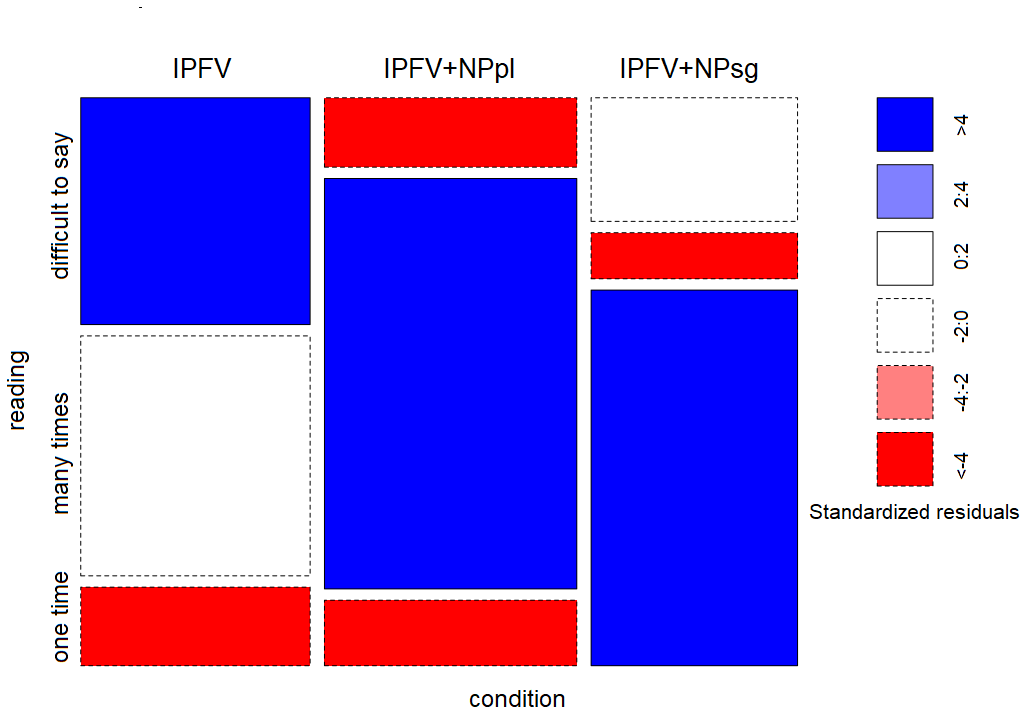
\includegraphics[scale=0.45]{mosaic_plot_ankiety.png}
\caption{Standardized residuals for three kinds of answers ‘one time’, ‘many times’, ‘it is hard to say as both readings are possible’ in three Conditions: \textsc{ipfv}, \textsc{ipfv}+NP$_\textsc{sg}$, \textsc{ipfv}+NP$_\textsc{pl}$.}\label{jan-bla:fansb:kb:fig1}
\end{figure}

\subsection{Discussion}\label{jan-bla:fansb:kb:sec3.3}

Taken together, when imperfective verbs were presented out of context, the answer ‘it is hard to say (both meanings are possible)’ was chosen more often than the remaining two answers ‘one time’ and ‘many times’. Only the difference between the number of ‘it is hard to say (both meanings are possible)’ and ‘one time’ readings was statistically significant. Additionally, the answer ‘many times’ was chosen significantly more often than the answer ‘one time’, which may suggest that the plural reading of imperfective aspect is dominant (more frequent). In contexts in which imperfective verbs were followed by a singular NP object, there was a significant preference for the ‘one time’ interpretation. Additionally, there was a significant preference for the ‘many times’ interpretation in contexts in which imperfective verbs were followed by a plural NP object. These data provide support for the claim that plural readings of imperfective verbs are obtained via a dependent reading between events described by a verb and individuals described by an NP object. Most importantly, the results of this study indicate that many respondents did not have a clear preference for any of the meanings of imperfective verbs presented out of context. For those respondents who had preferences, the plural event reading of bare imperfective verbs was preferred over the single ongoing reading. Additionally, the results indicate that the grammatical number of NP complements of imperfective verbs can serve as a contextual cue pointing to either the single ongoing or plural meaning of imperfective verbs. In order to account for the observations made in our online questionnaire study, in the following section we will adopt \citeauthor{Ferreira2004}'s (\citeyear{Ferreira2004, Ferreira2005}) number approach to imperfective aspect (which is compatible with \citeauthor{Kagan2008}'s \citeyear{Kagan2008, Kagan2010} view of imperfective aspect) and \citeposst{deSwart2006} notion of bijection.

\section{The number approach to imperfective aspect}\label{jan-bla:fansb:kb:sec4}

\subsection{\citeauthor{Ferreira2004}'s (\citeyear{Ferreira2004, Ferreira2005}) number approach to imperfective}\label{jan-bla:fansb:kb:sec4.1}

\citet{Ferreira2004, Ferreira2005} extends \citeposst{Link1983} original idea that the domain of individuals is formed by singular as well as plural objects (where singular objects are atomic entities and have no proper parts while plural objects are mereological sums having proper parts) and argues that a similar mereology can be extended to the domain of events. More precisely, \citet{Ferreira2004, Ferreira2005} argues that the singular/plural opposition used by \citet{Link1983} to distinguish between atomic and non-atomic individuals in the domain of objects applies to events as well with plural events being characterizable as mereological sums having singular events as their minimal parts. \citet{Ferreira2004, Ferreira2005} argues that imperfective aspect is an operator which selects for either plural or singular VPs: \textsc{ipfv} [VP$_\textsc{sg}$/VP$_\textsc{pl}$]. The single ongoing interpretation of an imperfective verb is derived from the logical form with the imperfective selecting for VP$_\textsc{sg}$, as presented in \REF{jan-bla:fansb:kb:ex11}.

\ea \sib{\textsc{ipfv}$_\textsc{sg}$} $= \lambda P_\cnst{sg}. \lambda t. \exists e : \tau(e) \supseteq t \wedge P(e)$\label{jan-bla:fansb:kb:ex11}
\z 

\noindent The plural event reading of an imperfective verb is derived from the logical form with the Imperfective selecting for VP$_\textsc{pl}$, as formally represented in \REF{jan-bla:fansb:kb:ex12}.

\ea \sib{\textsc{ipfv}$_\textsc{pl}$} $= \lambda P_\cnst{pl}. \lambda t. \exists e : \tau(e) \supseteq t \wedge P(e)$\label{jan-bla:fansb:kb:ex12}
\z 

\noindent \citet{Ferreira2004, Ferreira2005} accounts for the unbounded interpretation of imperfective aspect by assuming \citegen{Klein1995} time relational semantics, where the perspective time $t$ is included in the temporal trace of an event $\tau(e)$. This means that while interpreting imperfective aspect we take the perspective of an "insider", who sees a portion of an event from the inside and is oblivious to its endpoints (see \citealt{KazaninaandPhillips2003}). 

In order to formally capture the fact that under the plural event reading of imperfective each of the events in the plural set is distributed over separate time intervals, \citet{Ferreira2004, Ferreira2005} assumes that the domain of intervals D$_i$ contains singular and plural intervals and there is a homomorphism $\tau$ between the structured domain of events and the structured domain of intervals, so that for any events $e$, $e'$, $\tau (e\oplus e') = \tau(e)\oplus \tau(e')$ where $\tau(e)$ is the time of the event $e$. 

\subsection{\citeauthor{Kagan2008}'s (\citeyear{Kagan2008, Kagan2010}) number approach to the perfective/imperfective opposition}\label{jan-bla:fansb:kb:sec4.2}

\citet{Kagan2008, Kagan2010} also proposes a number approach to aspect but she draws an analogy between the singular/plural opposition in the nominal domain to the perfective/imperfective opposition in the verbal domain.\footnote{See also \citet{Rothstein2020} who, following \citet{Kagan2010}, treats ‟imperfective root verbs as plural predicates denoting sets of plural events, with singular events the borderline case of plurality” (p. 156).} Following \citet{Sauerland2003a}, \citet{Kagan2008, Kagan2010} assumes that the semantics of plural NPs is essentially neutral with respect to number, that is, the denotation of a bare plural NP contains both pluralities of objects and singular objects while the denotation of singular NPs which is restricted to atomic individuals, as shown in \REF{jan-bla:fansb:kb:ex13} and \REF{jan-bla:fansb:kb:ex14}.

\ea \sib{\textsc{sg}} $= \lambda P. \lambda x.P(x) \wedge \cnst{sng}(P) $\label{jan-bla:fansb:kb:ex13}
\z 

\ea \sib{\textsc{pl}} $= \lambda P. \lambda x.P(x) $\label{jan-bla:fansb:kb:ex14}
\z 

\noindent \citet{Kagan2008, Kagan2010} applies this semantics proposed for singular and plural morphology in the nominal domain to the perfective versus imperfective opposition, as demonstrated in \REF{jan-bla:fansb:kb:ex15} and \REF{jan-bla:fansb:kb:ex16}. 

\ea \sib{\textsc{pfv}} $= \lambda P. \lambda e.P(e) \wedge \cnst{sng}(P) $\label{jan-bla:fansb:kb:ex15}
\z 

\ea \sib{\textsc{ipfv}} $= \lambda P. \lambda e.P(e) $\label{jan-bla:fansb:kb:ex16}
\z 

\noindent More precisely, it is assumed that just like singular NPs denote singular object (atomic individuals), perfective predicates denote atomic events.\footnote{Following \citet{Krifka1992}, \citet{Filip2000} and \citet{Rothstein2004}, among others, it is assumed that atomicity or singularity involves quantization.} In a similar vein, just like the denotation of bare plural NPs contain both pluralities of objects and singular objects, the denotation of the imperfective aspect encompasses both atomic and non-atomic events. Thus, the imperfective aspect, just like the plural number, are treated as default in the proposed analysis.\footnote{As \citet{Kagan2010} points out, the view of the imperfective as a default aspect is by no means new. Similar observations can be found in the literature already in  \citet{Forsyth1970}.}\textsuperscript{,}\footnote{The choice of a specific aspect form of a verb in a given context is claimed to be pragmatic in nature. More precisely, it is assumed to be subject to the Gricean Maxim of Quantity, which \citet{Kagan2008, Kagan2010} is defined following \citet{Sauerland2003b} as follows:	a.	Maximize Assertion: Use the most informative assertion that is true. b.	Maximize Presupposition: Use the most informative presupposition that is satisfied.   
Since, as revealed in \REF{jan-bla:fansb:kb:ex16}, a perfective form is more restricted in meaning than its imperfective counterpart, whenever the former is appropriate (as contributing an entailment that the event described by the speaker is atomic), the use of the latter is ruled out by the above principles. The choice of the less restricted imperfective form thus triggers a conclusion on the part of the hearer that the perfective form was not appropriate. In other words, the hearer can conclude in this case that ‟atomicity requirement is not satisfied, or at least that the speaker does not have sufficient evidence that the event she has encoded is indeed atomic” \citep[pp. 10-12]{Kagan2008}.}
 
What is crucial in \citeauthor{Kagan2008}'s (\citeyear{Kagan2008, Kagan2010}) approach is that the imperfective is number neutral and its interpretation is determined on the basis of Gricean maxims while \citet{Ferreira2004, Ferreira2005} claims that the imperfective operator selects either a singular or a plural VP. \citet{Ferreira2004, Ferreira2005} does not specify which factors determine the selection. We think that his approach leaves more room for capturing the role of the grammatical number of NP objects in the selection of a plural or singular event.  

\subsection{A preliminary proposal}\label{jan-bla:fansb:kb:sec4.3}

In our study we adopt \citeauthor{Ferreira2004}'s (\citeyear{Ferreira2004, Ferreira2005}) number approach to imperfective aspect and we extend it by adopting \citeposst{Dolling2014} underspecification approach (which will be discussed later in this section). We argue that imperfective verbs are underspecified for number (they are underspecified for whether they denote singular or plural eventualities). When combined with time-relational semantics, perfective verbs refer to single bounded eventualities and imperfective verbs refer to single or plural temporally unbounded eventualities. As revealed by the results of the online questionnaire reported in \sectref{jan-bla:fansb:kb:sec3}, the grammatical number of NP complements of imperfective verbs can serve as a contextual cue pointing to either the single ongoing or plural meaning of imperfective verbs. Consider examples \REF{jan-bla:fansb:kb:ex4} and \REF{jan-bla:fansb:kb:ex5} presented earlier in the introduction and repeated here for convenience as \REF{jan-bla:fansb:kb:ex17} and \REF{jan-bla:fansb:kb:ex18}. 

\ea
\gll Rubens malował kobietę.\\  
     Rubens paint.\textsc{ipfv}.\textsc{pst}.\textsc{3sg}.\textsc{m} woman.\textsc{sg}.\textsc{acc}\\\hfill = \REF{jan-bla:fansb:kb:ex4}
\glt ‘Rubens was painting a woman.’\label{jan-bla:fansb:kb:ex17}
\z

\ea
\gll Rubens malował kobiety.\\  
     Rubens paint.\textsc{ipfv}.\textsc{pst}.\textsc{3sg}.\textsc{m} woman.\textsc{pl}.\textsc{acc}\\\hfill = \REF{jan-bla:fansb:kb:ex5}
\glt ‘Rubens painted women.’\label{jan-bla:fansb:kb:ex18}
\z

\noindent Assuming following \citet{Ferreira2004, Ferreira2005} that an imperfective operator selects for either singular or plural VPs, the sentences in \REF{jan-bla:fansb:kb:ex17} and \REF{jan-bla:fansb:kb:ex18} have two possible contextual interpretations each, one with a singular event e and one with a plural event $E$ (note that $x$ is used to represent singular individuals and $X$ is used to represent plural individuals), as presented in \REF{jan-bla:fansb:kb:ex19}--\REF{jan-bla:fansb:kb:ex26}.

\ea $\exists e \exists x [\textsc{paint}(e) \wedge \cnst{agent} (\textsc{Rubens}, e) \wedge \textsc{woman}(x) \wedge \cnst{theme} (e) = x]$\label{jan-bla:fansb:kb:ex19}
\z

\begin{figure}[H]
\begin{tikzpicture}[every node/.style={inner sep=0pt}]
% left ellipsis nodes
\node (e1) {\strut};
\node (e2) [below of=e1] {$e_1$\strut};
\node (e3) [below of=e2] {\strut};
%spacers (empty)
\node (eX) [left=2mm of e2] {\strut};
\node (eY) [right=2mm of e2] {\strut};
% left label
\node (e) [above = 8mm of e1] {$e$};
% right ellipsis nodes
\node (x0) [right=3cm of e1] {\strut};
\node (x1) [right=3cm of e2] {$x_1$\strut};
\node (x2) [right=3cm of e3] {\strut};
%spacers (empty)
\node (xX) [left=2mm of x1] {};
\node (xY) [right=2mm of x1] {};
%right label
\node (x)  [right=3cm of  e] {~$x$};
%ellipses
\node[fit=(e1)(e3)(eX)(eY), shape=ellipse, draw] {};
\node[fit=(x0)(x2)(xX)(xY), shape=ellipse, draw] {}; 
%arrows
% \draw[-latex] (e1) -- (x1);
\draw[-latex] (e2) -- (x1);
% \draw[-latex] (e3) -- (x1);
\end{tikzpicture}
% 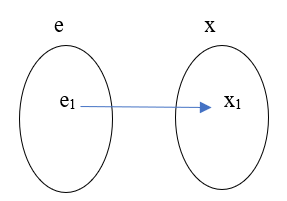
\includegraphics[scale=0.5]{j1.png}
\caption{Contextual single event interpretations of the sentence in (17)}
\end{figure}

\ea $\exists E \exists x [\textsc{paint}(E) \wedge \cnst{agent} (\textsc{Rubens}, E) \wedge \textsc{woman}(x) \wedge \cnst{theme} (E) = x]$\label{jan-bla:fansb:kb:ex20}
\z

\begin{figure}[H]
\begin{tikzpicture}[every node/.style={inner sep=0pt}]
% left ellipsis nodes
\node (e1) {$e_1$\strut};
\node (e2) [below of=e1] {$e_2$\strut};
\node (e3) [below of=e2] {$e_3$\strut};
%spacers (empty)
\node (eX) [left=2mm of e2] {\strut};
\node (eY) [right=2mm of e2] {\strut};
% left label
\node (E) [above = 8mm of e1] {$E$};
% right ellipsis nodes
\node (x0) [right=3cm of e1] {\strut};
\node (x1) [right=3cm of e2] {$x_1$\strut};
\node (x2) [right=3cm of e3] {\strut};
%spacers (empty)
\node (xX) [left=2mm of x1] {};
\node (xY) [right=2mm of x1] {};
%right label
\node (x)  [right=3cm of  E] {~$x$};
%ellipses
\node[fit=(e1)(e3)(eX)(eY), shape=ellipse, draw] {};
\node[fit=(x0)(x2)(xX)(xY), shape=ellipse, draw] {}; 
%arrows
\draw[-latex] (e1) -- (x1);
\draw[-latex] (e2) -- (x1);
\draw[-latex] (e3) -- (x1);
\end{tikzpicture}
% 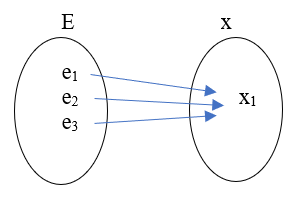
\includegraphics[scale=0.5]{j2.png}
\caption{Contextual plural event interpretations of the sentence in (17)}
\end{figure}

\ea $\exists e \exists X [\textsc{paint}(e) \wedge \cnst{agent} (\textsc{Rubens}, e) \wedge \textsc{woman}(X) \wedge \cnst{theme} (e) = X]$\label{jan-bla:fansb:kb:ex21}
\z

\begin{figure}[H]
\begin{tikzpicture}[every node/.style={inner sep=0pt}]
% right ellipsis nodes
\node (x0)  {$x_1$\strut};
\node (x1) [below of=x0] {$x_2$\strut};
\node (x2) [below of=x1] {$x_3$\strut};
%spacers (empty)
\node (xX) [left=2mm of x1] {};
\node (xY) [right=2mm of x1] {};
%right label
\node (x)  [above=8mm of x0] {~$X$};
% left ellipsis nodes
\node (e1) [left=3cm of x0] {\strut};
\node (e2) [left=3cm of x1] {$e_1$\strut};
\node (e3) [left=3cm of x2] {\strut};
%spacers (empty)
\node (eX) [left=2mm of e2] {\strut};
\node (eY) [right=2mm of e2] {\strut};
% left label
\node (E) [left = 3cm of x] {$e$};
%ellipses
\node[fit=(e1)(e3)(eX)(eY), shape=ellipse, draw] {};
\node[fit=(x0)(x2)(xX)(xY), shape=ellipse, draw] {}; 
%arrows
\draw[-latex] (e2) -- (x0);
\draw[-latex] (e2) -- (x1);
\draw[-latex] (e2) -- (x2);
\end{tikzpicture}
% 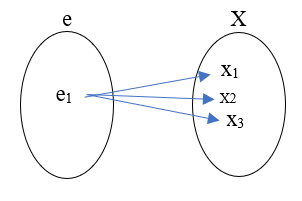
\includegraphics[scale=0.5]{j3.png}
\caption{Contextual single event interpretations of the sentence in (18)}
\end{figure}

\ea $\exists E \exists X [\textsc{paint}(E) \wedge \cnst{agent} (\textsc{Rubens}, E) \wedge \textsc{woman}(X) \wedge \cnst{theme} (E) = X \wedge f: E \leftrightarrow X]$\label{jan-bla:fansb:kb:ex22}
\z

\noindent $E \leftrightarrow X$ represents a bijection (one-to-one) relation between members of the plural event $E$ (understood as a sum of events) and the members of the plural entity $X$ (understood as a sum of individuals).

\begin{figure}[H]
\begin{tikzpicture}[every node/.style={inner sep=0pt}]
% right ellipsis nodes
\node (x0)  {$x_1$\strut};
\node (x1) [below of=x0] {$x_2$\strut};
\node (x2) [below of=x1] {$x_3$\strut};
%spacers (empty)
\node (xX) [left=2mm of x1] {};
\node (xY) [right=2mm of x1] {};
%right label
\node (x)  [above=8mm of x0] {~$X$};
% left ellipsis nodes
\node (e1) [left=3cm of x0] {$e_1$\strut};
\node (e2) [left=3cm of x1] {$e_2$\strut};
\node (e3) [left=3cm of x2] {$e_3$\strut};
%spacers (empty)
\node (eX) [left=2mm of e2] {\strut};
\node (eY) [right=2mm of e2] {\strut};
% left label
\node (E) [left = 3cm of x] {$E$};
%ellipses
\node[fit=(e1)(e3)(eX)(eY), shape=ellipse, draw] {};
\node[fit=(x0)(x2)(xX)(xY), shape=ellipse, draw] {}; 
%arrows
\draw[-latex] (e1) -- (x0);
\draw[-latex] (e2) -- (x1);
\draw[-latex] (e3) -- (x2);
\end{tikzpicture}
% 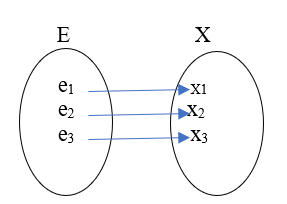
\includegraphics[scale=0.5]{j4.png}
\caption{Contextual plural event interpretations of the sentence in (18)}
\end{figure}

This means that the sentence in \REF{jan-bla:fansb:kb:ex17} with an imperfective verb and a singular NP object is in principle ambiguous between the interpretations represented in \REF{jan-bla:fansb:kb:ex19} and \REF{jan-bla:fansb:kb:ex20}. However, the interpretation in \REF{jan-bla:fansb:kb:ex20} where there is a plural event of Ruben’s painting the same woman is pragmatically implausible, therefore the interpretation in \REF{jan-bla:fansb:kb:ex19} is strongly preferred. Similarly, the sentence in \REF{jan-bla:fansb:kb:ex18} is ambiguous between the interpretations represented in \REF{jan-bla:fansb:kb:ex21} and \REF{jan-bla:fansb:kb:ex22} but the interpretation in \REF{jan-bla:fansb:kb:ex21} where there is a single event of Rubens’ painting multiple women is pragmatically implausible, therefore the interpretation in \REF{jan-bla:fansb:kb:ex22} is strongly preferred. The configuration in \REF{jan-bla:fansb:kb:ex22} is the only one in which there are two plural sums and it is possible to establish a bijection (one-to-one) relation between members of the plural event $E$ (understood as a sum of events) and members of the plural entity $X$ (understood as a sum of individuals) giving rise to a dependent reading between pairs of individuals (denoted by an NP$_\textsc{pl}$) and events (denoted by a VP$_\textsc{pl}$). Given the results of our questionnaire study, it appears to be the case that in most scenarios it is pragmatically more plausible that plural events involve different entities which disfavors or even blocks the use of singular NP objects under the plural event reading of imperfective. However, there are contexts in which it is not impossible, as shown in \REF{jan-bla:fansb:kb:ex23}.

\ea\label{jan-bla:fansb:kb:ex23}
\gll Audrey Hepburn paliła fajkę.\\  
     Audrey Hepburn smoke.\textsc{ipfv.pst.3sg.f} pipe.\textsc{sg.acc}\\
\glt ‘Audrey Hepburn smoked a tobacco pipe.’
\z

\ea\label{jan-bla:fansb:kb:ex24}
\gll Audrey Hepburn paliła fajki.\\  
      Audrey Hepburn smoke.\textsc{ipfv}.\textsc{pst}.\textsc{3sg}.\textsc{f} pipe.\textsc{pl}.\textsc{acc}\\
\glt ‘Audrey Hepburn smoked tobacco pipes.’
\z

\noindent \REF{jan-bla:fansb:kb:ex23} can be exceptionally interpreted as describing a plural event of Audrey’s smoking the same pipe on each occasion because it is pragmatically possible to smoke the same pipe several times. By contrast, in \REF{jan-bla:fansb:kb:ex25} Sherlock’s smoking the same cigarette on different occasions is pragmatically odd, therefore the plural event reading in this scenario is more naturally expressed in \REF{jan-bla:fansb:kb:ex26} with a plural NP object allowing for a bijection relation between the set of events in the denotation of an imperfective verb and the set of individuals in the denotation of a plural NP object.  

\ea\label{jan-bla:fansb:kb:ex25}
\gll Sherlock Holmes palił papierosa.\\  
     Sherlock Holmes smoke.\textsc{ipfv}.\textsc{pst}.\textsc{3sg}.\textsc{m} tobacco-pipe.\textsc{sg}.\textsc{acc}\\
\glt ‘Sherlock Holmes smoked a cigarette.’
\z

\ea\label{jan-bla:fansb:kb:ex26}
\gll Sherlock Holmes palił papierosy.\\  
     Sherlock Holmes smoke.\textsc{ipfv}.\textsc{pst}.\textsc{3sg}.\textsc{m} cigarettes.\textsc{pl}.\textsc{acc}\\
\glt ‘Sherlock Holmes smoked cigarettes.’
\z

\noindent It thus appears to be the case that the number approach to imperfective aspect alone is insufficient to account for the interaction between imperfective aspect and the number of NP objects as it is to a large extent a result of the interaction of semantics and pragmatics. For this reason we would like to propose that the two independent approaches to imperfective aspect: the underspecification approach (see \sectref{jan-bla:fansb:kb:sec2}) and the number approach (as presented in the present section) should be combined and that is reasonable to assume that imperfective aspect is underspecified for number. This can be elegantly captured in more formal terms by adopting the model of interpretation of aspectually underspecified representations proposed by \citet{Dolling2014} and \citet{Egg2005}, which is presented in the next section.

\section{The proposed model of interpretation of imperfective aspect}\label{jan-bla:fansb:kb:sec5}

A theoretical approach to resolving semantically underspecified expressions, also in the aspectual domain, has been proposed by \citet{Dolling1995, Dolling1997, Dolling2001, Dolling2003b,Dolling2003a, Dolling2014} and \citet{Egg2005}, among others.  In a nutshell, it is assumed that the computation of a fully specified meaning takes place in two steps (see also the two-level semantic approach by \citealt{Bierwisch1983, Bierwisch1997, Bierwisch2007}; \citealt{BierwishandLang1989}; \citealt{BierwischandSchreuder1992}; \citealt{Lang1994}). The first step consists in the computation of an underspecified representation in a strictly compositional fashion. Crucially, in the first step everything which needs further disambiguation is left open. More specifically, \citet{Egg2005} proposes that semantic representation introduces particular gaps or blanks which can be filled in with relevant aspectual operators in order to buffer aspectual conflicts. \citet{Dolling2014} claims that in the first stage an abstract, underspecified coercion operator is mandatorily inserted in semantic composition. The disambiguation of an underspecified representation is part of the second computational step. It is based on pragmatic information such as discourse context or conceptual knowledge. In Egg’s work aspectual mismatches, for example, are resolved by inserting an appropriate operator (e.g., iteration, add preparation etc.) into the underspecified representation, whereby the choice of an operator is determined on pragmatic grounds. In \citet{Dolling2014}, in the second step an aspectual coercion can be realized by pragmatically enriching it. However, as \citet[p. 47]{Bott2010} points out, “[l]ike the previous accounts, \citet{ Egg2005} does not provide a theory of how and when pragmatic information is brought into the specification process.” 

Inspired by the works of \citet{Dolling2014} and \citet{Egg2005}, we propose that upon encountering an imperfective predicate, the \textsc{ipfv} operator is added to the semantic representation and it is underspecified for number. Importantly, we assume, following \citet{Tatevosov2011, Tatevosov2015}, that the aspectual operators \textsc{ipfv} and \textsc{pfv} act at the level of AspP (and are phonologically null) and their morphological exponents merge lower in the syntactic hierarchy. We adopt \citeauthor{Dolling2014}'s (\citeyear[34--35]{Dolling2014}) formalism, according to which each verbal predicate is added to the representation with a template called \textsc{coerce}, which has the following form $\lambda P \lambda e. Qe': R(e', e) [P(e')]$ (an abstract coercion operator) and which denotes a mapping from properties of eventualities of a certain sort onto properties of eventualities of some other sort. More precisely, properties $P$ are mapped onto properties $\lambda e. Qe': R(e', e) [P(e')]$ where some quantifier Q (which can be instantiated as $\exists$ or $\forall$) ranging over $e'$ has as its restriction an inter-sortal relation $R$ between $e'$ and $e$, and its scope is the proposition that $e'$ is $P$. The symbol $R$ can be instantiated by any inter-sortal relation between eventualities understood as shifts from one aspectual type to another. In \citeauthor{Dolling2014}'s (\citeyear[34--35]{Dolling2014}) formalism the fixation of the parameter $R$ is left to context and it involves a pragmatic enrichment mechanism. As a consequence, the template \textsc{coerce} leaves room for different specifications at the pragmatics-semantics interface. \citet[34--35]{Dolling2014} illustrates the use of the \textsc{coerce} template in the VP \textit{play the sonata} (see \REF{jan-bla:fansb:kb:ex27}), which can be coerced into a repetitive action of playing the same sonata over and over again when combined with a temporal adverbial specifying a long temporal interval.

\ea \sib{play the sonata}: $\lambda e. \textsc{play}(e) \wedge \cnst{theme}(\textsc{the sonata}, e)$\label{jan-bla:fansb:kb:ex27}
\z

\ea \textsc{coerce}: 
$\lambda P \lambda e.Qe': R(e', e) [P(e')]$\label{jan-bla:fansb:kb:ex28}
\z

\ea \sib{play the sonata}: $\lambda e.Qe': R(e',e) [\textsc{play}(e') \wedge \cnst{theme}(\textsc{the sonata}, e')]$\label{jan-bla:fansb:kb:ex29}
\z

\noindent We would like to propose that Dölling’s (2014) \textsc{coerce} template is an obligatory element of the semantics of the imperfective operator, as represented in \REF{jan-bla:fansb:kb:ex28}:

\ea \sib{\textsc{ipfv}} $= \lambda P. \lambda t.\lambda e. \exists e' [\cnst{numb} (e, e') \wedge t \subseteq \tau(e') \wedge P(e')=1]$\label{jan-bla:fansb:kb:ex30}
\z 

\noindent The \textsc{coerce} template involves a number operator \cnst{numb}, which maps singular or plural eventualities to their plural or singular counterparts. Inspired by the insights of recent psycholinguistic studies related to the processing of polysemous lexical items (\citealt{KleinandMurphy2002}; \citealt{PylkkänenLlinásandMurphy2006}; \citealt{Frisson2015}), we assume that the plural and singular readings of events are listed as separate senses of verbal lexical entries. More precisely, we think that these senses (singular/plural) are connected to the same abstract lexical representation of a given verbal predicate but the senses themselves are distinctly listed and some of them may be more dominant (more frequent) than others.  Most predicates such as \textit{palić} ‘smoke’, \textit{gotować} ‘cook’, \textit{sprzątać} ‘clean’, \textit{uczyć} ‘teach’, \textit{myć} ‘wash’, \textit{jeść} ‘eat’ (and the predicates used in our questionnaire) have a more dominant (more frequent) plural event sense because they are more often used in plural event contexts. In the case of such predicates, when the context supports the singular event reading, the number operator in the \textsc{coerce} template takes as its input a more dominant plural eventuality and it switches it to a singular event reading. However, there are also predicates which describe eventualities which normally do not happen regularly such as \textit{rodzić} ‘give birth’, \textit{umierać} ‘die’ because they are more often used as episodic events. The dominant sense of such predicates is a singular event. In the case of these predicates, when the context supports the plural event reading, the number operator in the \textsc{coerce} template maps a singular eventuality to a plural one. In psycholinguistic research, it has been shown that sense frequency has an impact on the interpretation process of polysemous words. It has been shown that switching between word senses under the influence of context is costly (see \citealt{Frisson2015} and the references mentioned therein). We think these context-dependent switches between singular and plural event senses of verbal predicates can be nicely captured formally by applying \citeposst{Dolling2014} \textsc{coerce} template, which acts at the semantics--pragmatics interface.

It may happen however that the dominant meaning (plural or singular) of an imperfective verb is consistent with context and no coercion is necessary. In such cases, we assume following \citet{Dolling2014} that the representation involves an equation between e and e’ which results in removing the \cnst{numb} operator as it involves an identity relation, as shown in \REF{jan-bla:fansb:kb:ex29}:

\ea \sib{\textsc{ipfv}} $= \lambda P. \lambda t.\lambda e. \exists e': e'=e [t \subseteq \tau(e') \wedge P(e')=1] 
\ \equiv \lambda P. \lambda t.\lambda e. [t \subseteq \tau(e') \wedge P(e')]$\label{jan-bla:fansb:kb:ex31}
\z 

\noindent Depending on the interaction with the surrounding context, the imperfective operator \textsc{ipfv} can thus be specified (via coercion) to a singular or plural event reading. The number of an NP object plays a crucial role in this specification process. As the results of our online questionnaire indicate, without any context, an imperfective verb can be interpreted as denoting a single event or multiple events, though its plural reading seems to be the dominant (more frequent) one. A plural event interpretation is strongly preferred with imperfective verbs followed by a plural NP object. By contrast, when an imperfective verb is followed by a singular NP object, there is a strong preference for a single event interpretation. This is especially the case with consumption verbs, as, for example, \textit{jeść jabłko} ‘to eat.\textsc{ipfv} an apple’, which cannot receive a ‘many times’ interpretation since with strong incremental theme verbs the participants of repeated events cannot be identical. In contrast, with verbs like, for example, \textit{podlewać ogród} ‘to water.\textsc{ipfv} a/the garden’ or \textit {reparować rower} ‘to repair.\textsc{ipfv} a/the bike’, a plural event interpretation, involving one and the same participant, is possible. This shows that the role of the number of NP objects is not deterministic in the specification process as it interacts with the information about the specific lexical semantics of a given imperfective verb. Furthermore, as we have seen in \sectref{jan-bla:fansb:kb:sec4}, the information about the number of an NP object also interacts with pragmatics or world knowledge.\footnote{As pointed out by an anonymous reviewer, it is very difficult to propose a theory of how and when pragmatic information is brought into the specification process of \textsc{ipfv}. The weak point of the present analysis is that there is a thin line between cases in which the “switching mode” of \textsc{coerce} (from a dominant plural sense to a singular one) is activated (as in Rubens painting the same woman again and again, which is pragmatically implausible since it is common knowledge that he painted different women on different occasions). In contrast to Audrey’s smoking the same pipe again and again, which is claimed to be pragmatically possible and leaves \textsc{coercion} in the “identity mode”. We think that it is necessary to investigate the role of singular/plural sense dominance of different imperfective verbs in the specification process to sort out the exact interplay of the \textsc{coerce} function of \textsc{ipfv}, sense dominance, the number of an NP object and pragmatics (world knowledge). 
} While a single unbounded event interpretation of an imperfective verb followed by a singular object might be more plausible in one case (recall the Rubens example in \REF{jan-bla:fansb:kb:ex17}), in another case it might in fact be more plausible to assume that the imperfective verb followed by a singular object denotes a plural event (recall the Audrey Hepburn example in \REF{jan-bla:fansb:kb:ex23}). 

\section{Conclusion}\label{jan-bla:fansb:kb:sec6}

To sum up, there is solid evidence that imperfective aspect is semantically underspecified (recall \sectref{jan-bla:fansb:kb:sec2}). However, we have shown that the underspecification approach alone is not able to capture some crucial facts related to the interaction of imperfective aspect and the number of the NP objects, as revealed by the results of our online questionnaire study (\sectref{jan-bla:fansb:kb:sec3}). We have also argued that although these observations could potentially be accounted for by applying \citeauthor{Ferreira2004}'s (\citeyear{Ferreira2004}, \citeyear{Ferreira2005}) number approach to imperfective aspect, this theory is too rigorous and it does not capture the fact that the interaction of the number semantics of imperfective aspect with the number of NP objects clearly relies on pragmatics (\sectref{jan-bla:fansb:kb:sec4}). In the present paper we propose a model of interpretation of imperfective aspect which in some sense combines the underspecification approach and the number approach to imperfective aspect as it takes imperfective aspect to be underspecified for number (\sectref{jan-bla:fansb:kb:sec4.3}). More precisely, following the ideas put forward by \citet{Dolling2003b,Dolling2003a,Dolling2014} and \citet{Egg2005}, we argue that the imperfective operator that is added to the representation contains a \textsc{coerce} template with a number operator in it and it is specified for number on the basis of the interaction between the number semantics of the NP object, the imperfective aspect and context (\sectref{jan-bla:fansb:kb:sec5}). Our account leaves room for the interaction between the grammatical number of the NP object, pragmatics and plural and singular senses of verbs, which all play a nontrivial role in the specification process of imperfective aspect, which in our view is underspecified for number. However, this proposal should be treated as a pathway for further research as there are still many interesting questions left open. For example, it would be interesting to extend the proposed analysis with questions related to the role of different lexical aspectual classes of verbs, the interaction of the plural and singular readings of \textsc{ipfv} with quantifiers. What is also nonstandard in our analysis is the proposal that the selection of singular and plural meanings of \textsc{ipfv} is preceded by the activation of plural and singular senses of verbal predicates. Finally, the psychological plausibility of the existence of the \textsc{coerce} operator leading to meaning shifts between singular and plural readings of \textsc{ipfv} should be experimentally investigated, for example in relation to sense dominance. 

\section*{Abbreviations}

\begin{tabularx}{.5\textwidth}{@{}lX@{}}
\textsc{2}&second person\\
\textsc{3}&{third person}\\
\textsc{acc}&{accusative}\\
\textsc{f}&{feminine}\\
\textsc{gen}&{genitive}\\
\textsc{inf}&{infinitive}\\
\textsc{ins}&{instrumental}\\
\textsc{ipfv}&{imperfective}\\
\end{tabularx}%
\begin{tabularx}{.5\textwidth}{@{}lX@{}}
\textsc{m}&{masculine}\\
\textsc{neg}&{negation}\\
\textsc{pfv}&{perfective}\\
\textsc{pl}&{plural}\\
\textsc{pst}&{past tense}\\
\textsc{refl}&{reflexive}\\
\textsc{sg}&{singular}\\
\\
\end{tabularx}

\section*{Acknowledgements}

This work was supported by the OPUS 5 HS2 grant (DEC-2013/09/B/HS2/02763) from the Polish National Science Center (NCN). We would like to thank Wojciech Witkowski for his help with the statistical analysis.

\section*{Appendix: Summary of the responses of all the participants for all the tested items}

\begin{sidewaystable}
    \scriptsize 
    \fittable{
    \begin{tabular}{l>{\raggedright}p{5cm}rrrrrrrrrrrrrrrrrrrrrrrrr}
    \lsptoprule
condition&item&p1&p2&p3&p4&p5&p6&p7&p8&p9&p10&p11&p12&p13&p14&p15&p16&p17&p18&p19&p20&p21&p22&p23&p24&p25\\\midrule
\textsc{ipfv}&ratował `[he] rescued'&3&1&3&3&3&2&2&1&3&3&3&3&3&3&3&3&2&3&3&3&2&3&3&3&3\\
\textsc{ipfv}&drukował `[he] printed'&1&1&2&2&3&1&1&3&3&3&2&1&3&3&3&2&2&3&2&3&2&2&3&3&3\\
\textsc{ipfv}&nagrywał `[he] recorded'&3&1&2&2&2&3&2&1&3&3&1&1&3&2&3&2&2&3&2&3&2&2&2&3&3\\
\textsc{ipfv}&pakował `[he] packed'&1&1&2&2&3&2&2&1&1&3&2&3&3&1&3&2&2&3&2&3&2&2&2&3&3\\
\textsc{ipfv}&rozliczał `[he] calculated'&2&3&2&2&3&2&2&2&3&3&2&3&3&1&3&3&2&3&3&3&2&2&3&3&3\\
\textsc{ipfv}&oceniał `[he] evaluated'&2&1&2&2&3&2&2&2&1&3&2&3&3&2&3&2&3&3&2&2&2&2&2&3&3\\
\textsc{ipfv}&montował `[he] installed'&2&1&2&2&3&2&2&3&1&2&1&3&3&2&3&2&3&3&2&3&2&2&3&3&3\\
\textsc{ipfv}&wycinał `[he] cut out'&1&1&2&2&3&2&2&2&1&2&1&1&3&1&3&2&2&3&2&3&2&2&3&3&2\\
\textsc{ipfv}&omawiał `[he] discussed'&2&1&2&2&3&2&2&2&3&3&1&1&3&2&3&2&2&3&2&3&1&2&3&3&3\\
\textsc{ipfv}&poprawiał `[he] corrected'&2&1&2&2&3&2&2&2&3&3&1&1&3&2&3&2&2&3&2&2&1&2&3&3&3\\
\textsc{ipfv}+NPsg&testował maszynę\newline  `[he] tested (a) machine'&1&2&2&1&2&1&1&1&1&3&1&1&1&3&2&2&3&3&1&1&2&2&1&2&3\\
\textsc{ipfv}+NPsg&rysował portret\newline  `[he] drew (a) portrait'&1&1&2&1&2&1&1&1&1&1&1&1&1&1&2&2&1&1&1&1&1&1&1&1&2\\
\textsc{ipfv}+NPsg&wystawiał ocenę\newline  `[he] gave (a) grade'&1&3&2&1&1&2&1&3&3&3&1&1&1&1&1&2&2&1&1&1&3&2&2&1&2\\
\textsc{ipfv}+NPsg&podrabiał podpis\newline  `[he] counterfeited (a) signature'&1&1&2&2&2&1&1&1&1&1&1&1&1&1&1&2&2&1&3&1&2&1&3&1&3\\
\textsc{ipfv}+NPsg&usuwał usterkę\newline  `[he] removed (a) failure'&1&1&1&1&1&1&1&1&1&3&1&1&1&1&3&2&2&1&1&1&2&2&2&1&2\\
\textsc{ipfv}+NPsg&wysyłał paczkę\newline  `[he] shipped (a) package'&1&1&1&1&1&1&1&1&1&3&1&1&1&1&1&2&1&1&1&1&1&1&2&1&2\\
\textsc{ipfv}+NPsg&malował obraz\newline  `[he] painted (a) painting'&1&1&1&1&1&1&1&1&1&2&1&1&1&1&3&1&1&1&1&1&1&1&1&1&2\\
\textsc{ipfv}+NPsg&szkicował budynek\newline  `[he] sketched (a) building'&1&1&2&1&1&1&1&1&1&2&1&1&1&1&2&2&2&1&2&1&2&1&2&1&1\\
\textsc{ipfv}+NPsg&wyłudzał łapówkę\newline  `[he] extorted (a) bribe'&1&3&2&1&1&1&1&1&1&3&1&1&1&1&2&2&1&1&2&1&2&1&2&1&1\\
\textsc{ipfv}+NPsg&uszczelniał okno\newline  `[he] sealed (a) window'&1&1&1&1&1&1&1&1&1&2&1&1&2&1&1&1&1&1&2&1&2&1&2&1&2\\
\textsc{ipfv}+NPpl&zamiatał korytarze\newline  `[he] swept corridors'&3&2&3&3&3&3&2&3&2&3&3&3&3&3&3&3&3&3&3&3&2&3&3&3&3\\
\textsc{ipfv}+NPpl&wyceniał działki\newline  `[he] priced plots of land'&3&2&3&3&3&3&3&3&3&3&1&3&3&3&3&1&3&3&3&3&2&3&3&3&3\\
\textsc{ipfv}+NPpl&podlewał trawniki\newline  `[he] watered lawns'&1&3&3&3&2&3&3&3&3&3&3&3&3&3&3&3&2&3&1&3&2&3&3&3&3\\
\textsc{ipfv}+NPpl&sporządzał raporty\newline  `[he] made reports'&3&1&3&3&3&3&3&3&3&3&3&3&3&3&3&3&3&3&3&3&2&3&3&3&3\\
\textsc{ipfv}+NPpl&podrywał dziewczyny\newline  `[he] picked up girls'&3&3&3&3&3&3&3&3&3&3&2&3&3&3&3&3&2&3&2&3&2&3&3&3&3\\
\textsc{ipfv}+NPpl&wygłaszał wykłady\newline  `[he] delivered lectures'&3&3&3&3&3&3&3&3&3&3&3&3&3&3&3&3&3&3&3&3&3&3&3&3&3\\
\textsc{ipfv}+NPpl&naprawiał rowery\newline  `[he] repaied bikes'&3&3&3&3&3&3&3&3&3&3&3&3&3&3&3&3&3&3&3&3&2&3&3&3&3\\
\textsc{ipfv}+NPpl&wypełniał blankiety\newline  `[he] filled in forms'&3&3&2&3&3&1&2&3&3&3&3&3&3&3&3&3&3&3&2&3&1&3&3&3&3\\
\textsc{ipfv}+NPpl&ozdabiał wnętrza\newline  `[he] decorated interiors'&3&3&2&3&3&3&3&3&3&3&3&3&3&3&3&3&3&3&3&3&2&3&3&3&3\\
\textsc{ipfv}+NPpl&szacował straty\newline  `[he] estimated losses'&3&1&2&2&3&1&1&2&3&3&2&1&3&1&2&3&2&3&2&3&1&2&3&1&2\\
\lspbottomrule
    \end{tabular}
    }
    \caption{Responses: p=participant, 1=one time,\\ 2=difficult to say (both meanings are possible), 3=many times}
    \label{jan-bla:fansb:kb:tab4}
\end{sidewaystable}

{\sloppy\printbibliography[heading=subbibliography,notkeyword=this]}

\end{document}
